% Editable source for result.pdf, written by make_figures.py from run_github_38891404048/panel/result.json
\documentclass[tikz,border=6pt]{standalone}
\usepackage[T1]{fontenc}
\begin{document}
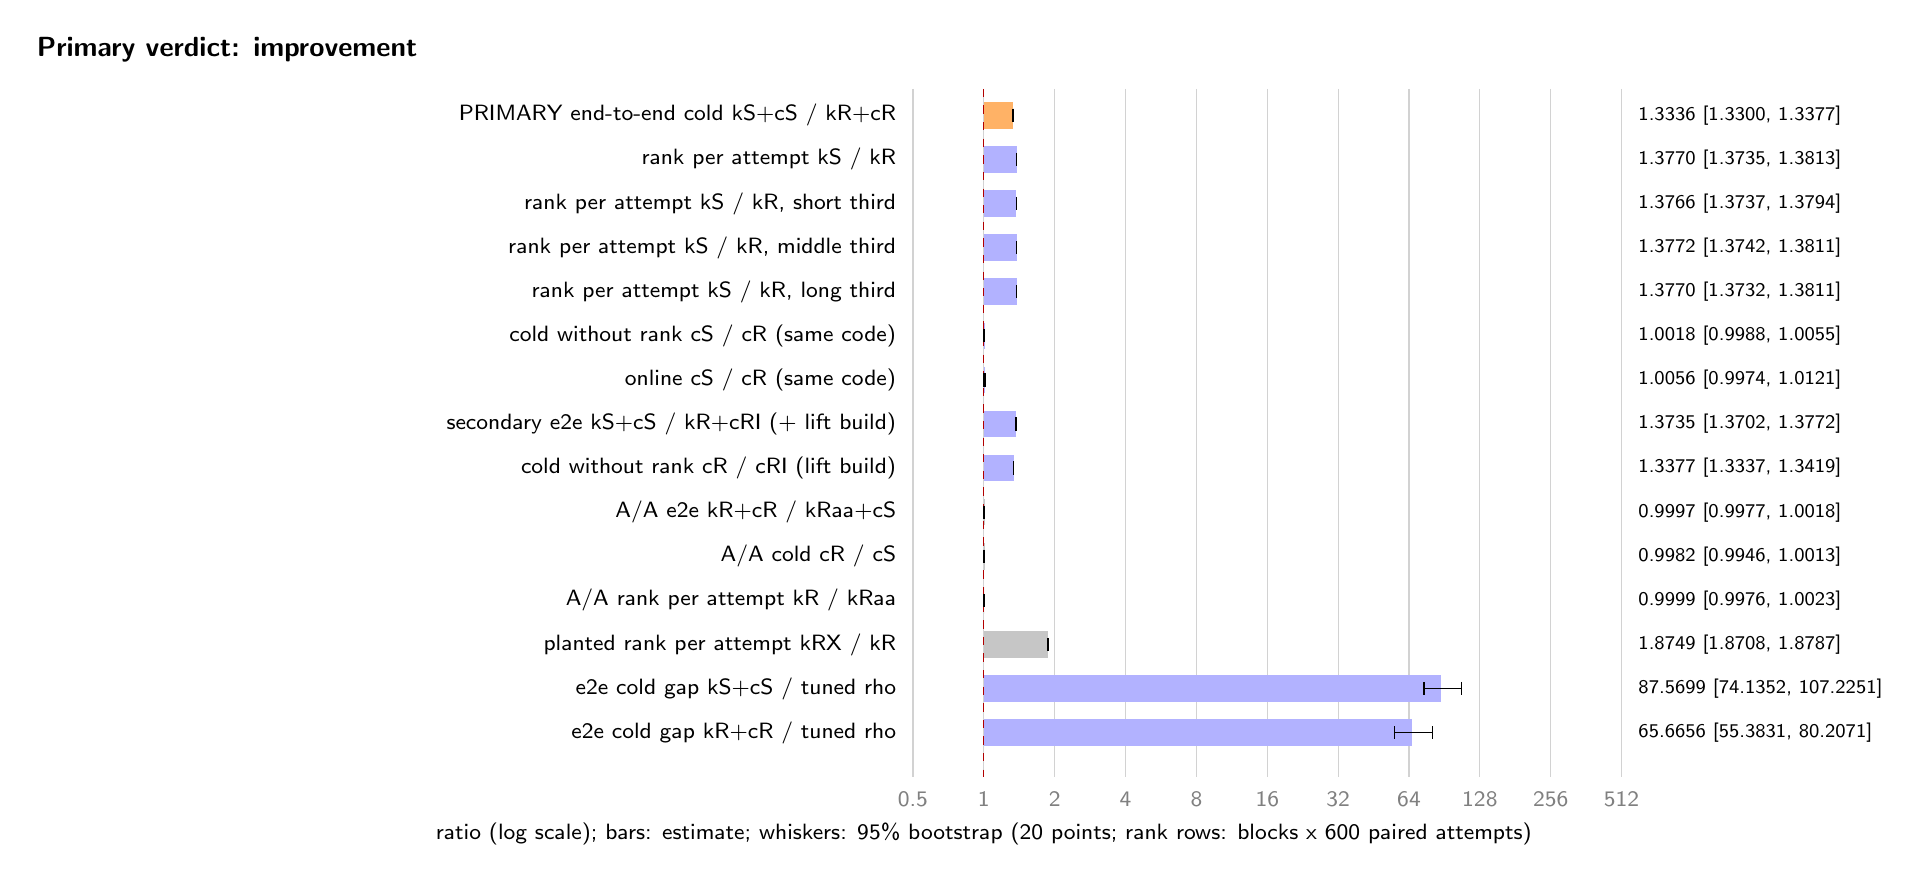
\begin{tikzpicture}[font=\sffamily\footnotesize,x=9mm,y=-5.6mm]
\draw[gray!35] (-1.0000,-0.6) -- (-1.0000,15); \node[gray] at (-1.0000,15.5) {0.5};
\draw[gray!35] (0.0000,-0.6) -- (0.0000,15); \node[gray] at (0.0000,15.5) {1};
\draw[gray!35] (1.0000,-0.6) -- (1.0000,15); \node[gray] at (1.0000,15.5) {2};
\draw[gray!35] (2.0000,-0.6) -- (2.0000,15); \node[gray] at (2.0000,15.5) {4};
\draw[gray!35] (3.0000,-0.6) -- (3.0000,15); \node[gray] at (3.0000,15.5) {8};
\draw[gray!35] (4.0000,-0.6) -- (4.0000,15); \node[gray] at (4.0000,15.5) {16};
\draw[gray!35] (5.0000,-0.6) -- (5.0000,15); \node[gray] at (5.0000,15.5) {32};
\draw[gray!35] (6.0000,-0.6) -- (6.0000,15); \node[gray] at (6.0000,15.5) {64};
\draw[gray!35] (7.0000,-0.6) -- (7.0000,15); \node[gray] at (7.0000,15.5) {128};
\draw[gray!35] (8.0000,-0.6) -- (8.0000,15); \node[gray] at (8.0000,15.5) {256};
\draw[gray!35] (9.0000,-0.6) -- (9.0000,15); \node[gray] at (9.0000,15.5) {512};
\draw[red!70!black,dashed] (0,-0.6) -- (0,15);
\node at (0,16.3) {ratio (log scale); bars: estimate; whiskers: 95\% bootstrap (20 points; rank rows: blocks x 600 paired attempts)};
\node[anchor=west,font=\sffamily\bfseries] at (-13.5,-1.5) {Primary verdict: improvement};
\node[anchor=east] at (-1.1000,0) {PRIMARY end-to-end cold kS+cS / kR+cR};
\fill[orange!60] (0,-0.300000) rectangle (0.4153,0.300000);
\draw (0.4115,0) -- (0.4198,0); \draw (0.4115,-0.150000) -- (0.4115,0.150000); \draw (0.4198,-0.150000) -- (0.4198,0.150000);
\node[anchor=west,font=\sffamily\scriptsize] at (9.1000,0) {1.3336 [1.3300, 1.3377]};
\node[anchor=east] at (-1.1000,1) {rank per attempt kS / kR};
\fill[blue!30] (0,0.700000) rectangle (0.4616,1.300000);
\draw (0.4579,1) -- (0.4661,1); \draw (0.4579,0.850000) -- (0.4579,1.150000); \draw (0.4661,0.850000) -- (0.4661,1.150000);
\node[anchor=west,font=\sffamily\scriptsize] at (9.1000,1) {1.3770 [1.3735, 1.3813]};
\node[anchor=east] at (-1.1000,2) {rank per attempt kS / kR, short third};
\fill[blue!30] (0,1.700000) rectangle (0.4611,2.300000);
\draw (0.4581,2) -- (0.4641,2); \draw (0.4581,1.850000) -- (0.4581,2.150000); \draw (0.4641,1.850000) -- (0.4641,2.150000);
\node[anchor=west,font=\sffamily\scriptsize] at (9.1000,2) {1.3766 [1.3737, 1.3794]};
\node[anchor=east] at (-1.1000,3) {rank per attempt kS / kR, middle third};
\fill[blue!30] (0,2.700000) rectangle (0.4618,3.300000);
\draw (0.4586,3) -- (0.4658,3); \draw (0.4586,2.850000) -- (0.4586,3.150000); \draw (0.4658,2.850000) -- (0.4658,3.150000);
\node[anchor=west,font=\sffamily\scriptsize] at (9.1000,3) {1.3772 [1.3742, 1.3811]};
\node[anchor=east] at (-1.1000,4) {rank per attempt kS / kR, long third};
\fill[blue!30] (0,3.700000) rectangle (0.4615,4.300000);
\draw (0.4576,4) -- (0.4658,4); \draw (0.4576,3.850000) -- (0.4576,4.150000); \draw (0.4658,3.850000) -- (0.4658,4.150000);
\node[anchor=west,font=\sffamily\scriptsize] at (9.1000,4) {1.3770 [1.3732, 1.3811]};
\node[anchor=east] at (-1.1000,5) {cold without rank cS / cR (same code)};
\fill[blue!30] (0,4.700000) rectangle (0.0026,5.300000);
\draw (-0.0018,5) -- (0.0079,5); \draw (-0.0018,4.850000) -- (-0.0018,5.150000); \draw (0.0079,4.850000) -- (0.0079,5.150000);
\node[anchor=west,font=\sffamily\scriptsize] at (9.1000,5) {1.0018 [0.9988, 1.0055]};
\node[anchor=east] at (-1.1000,6) {online cS / cR (same code)};
\fill[blue!30] (0,5.700000) rectangle (0.0081,6.300000);
\draw (-0.0038,6) -- (0.0173,6); \draw (-0.0038,5.850000) -- (-0.0038,6.150000); \draw (0.0173,5.850000) -- (0.0173,6.150000);
\node[anchor=west,font=\sffamily\scriptsize] at (9.1000,6) {1.0056 [0.9974, 1.0121]};
\node[anchor=east] at (-1.1000,7) {secondary e2e kS+cS / kR+cRI (+ lift build)};
\fill[blue!30] (0,6.700000) rectangle (0.4579,7.300000);
\draw (0.4544,7) -- (0.4617,7); \draw (0.4544,6.850000) -- (0.4544,7.150000); \draw (0.4617,6.850000) -- (0.4617,7.150000);
\node[anchor=west,font=\sffamily\scriptsize] at (9.1000,7) {1.3735 [1.3702, 1.3772]};
\node[anchor=east] at (-1.1000,8) {cold without rank cR / cRI (lift build)};
\fill[blue!30] (0,7.700000) rectangle (0.4197,8.300000);
\draw (0.4154,8) -- (0.4243,8); \draw (0.4154,7.850000) -- (0.4154,8.150000); \draw (0.4243,7.850000) -- (0.4243,8.150000);
\node[anchor=west,font=\sffamily\scriptsize] at (9.1000,8) {1.3377 [1.3337, 1.3419]};
\node[anchor=east] at (-1.1000,9) {A/A e2e kR+cR / kRaa+cS};
\fill[gray!45] (0,8.700000) rectangle (-0.0004,9.300000);
\draw (-0.0033,9) -- (0.0026,9); \draw (-0.0033,8.850000) -- (-0.0033,9.150000); \draw (0.0026,8.850000) -- (0.0026,9.150000);
\node[anchor=west,font=\sffamily\scriptsize] at (9.1000,9) {0.9997 [0.9977, 1.0018]};
\node[anchor=east] at (-1.1000,10) {A/A cold cR / cS};
\fill[gray!45] (0,9.700000) rectangle (-0.0026,10.300000);
\draw (-0.0078,10) -- (0.0019,10); \draw (-0.0078,9.850000) -- (-0.0078,10.150000); \draw (0.0019,9.850000) -- (0.0019,10.150000);
\node[anchor=west,font=\sffamily\scriptsize] at (9.1000,10) {0.9982 [0.9946, 1.0013]};
\node[anchor=east] at (-1.1000,11) {A/A rank per attempt kR / kRaa};
\fill[gray!45] (0,10.700000) rectangle (-0.0001,11.300000);
\draw (-0.0034,11) -- (0.0033,11); \draw (-0.0034,10.850000) -- (-0.0034,11.150000); \draw (0.0033,10.850000) -- (0.0033,11.150000);
\node[anchor=west,font=\sffamily\scriptsize] at (9.1000,11) {0.9999 [0.9976, 1.0023]};
\node[anchor=east] at (-1.1000,12) {planted rank per attempt kRX / kR};
\fill[gray!45] (0,11.700000) rectangle (0.9068,12.300000);
\draw (0.9037,12) -- (0.9097,12); \draw (0.9037,11.850000) -- (0.9037,12.150000); \draw (0.9097,11.850000) -- (0.9097,12.150000);
\node[anchor=west,font=\sffamily\scriptsize] at (9.1000,12) {1.8749 [1.8708, 1.8787]};
\node[anchor=east] at (-1.1000,13) {e2e cold gap kS+cS / tuned rho};
\fill[blue!30] (0,12.700000) rectangle (6.4524,13.300000);
\draw (6.2121,13) -- (6.7445,13); \draw (6.2121,12.850000) -- (6.2121,13.150000); \draw (6.7445,12.850000) -- (6.7445,13.150000);
\node[anchor=west,font=\sffamily\scriptsize] at (9.1000,13) {87.5699 [74.1352, 107.2251]};
\node[anchor=east] at (-1.1000,14) {e2e cold gap kR+cR / tuned rho};
\fill[blue!30] (0,13.700000) rectangle (6.0371,14.300000);
\draw (5.7914,14) -- (6.3257,14); \draw (5.7914,13.850000) -- (5.7914,14.150000); \draw (6.3257,13.850000) -- (6.3257,14.150000);
\node[anchor=west,font=\sffamily\scriptsize] at (9.1000,14) {65.6656 [55.3831, 80.2071]};
\end{tikzpicture}
\end{document}
